\documentclass{article}

% Language setting
% Replace `english' with e.g. `spanish' to change the document language
\usepackage[italian]{babel}
\usepackage{siunitx}
\usepackage{graphicx}
\usepackage{gensymb}
\usepackage{setspace}
\setstretch{1.5}

% Set page size and margins
% Replace `letterpaper' with`a4paper' for UK/EU standard size
\usepackage[letterpaper,top=2cm,bottom=2cm,left=3cm,right=3cm,marginparwidth=1.75cm]{geometry}

% Useful packages
\usepackage{amsmath}
\usepackage{graphicx}
\usepackage[colorlinks=true, allcolors=blue]{hyperref}

\title{
Controllo satellite in orbita intorno alla Terra\\
  \large Progetto Tipologia b - Traccia 2 \\
Controlli Automatici - T

}

\author{A cura di : Giorgio Mastrotucci, Lorenzo Venerandi e Patrick Di Fazio}
\date{}
\begin{document}
\maketitle

\begin{abstract}
\begin{figure}[h!]
\centering
\includegraphics[width=0.3\textwidth]{Schermata 2022-02-04 alle 19.54.38.png}
\caption{\label{fig:orbit}Schema illustrativo della dinamica del satellite}
\end{figure}
\end{abstract}

\begin{center}
\section*{Descrizione del problema}
\end{center}
Il progetto richiede di realizzare un sistema di controllo per un satellite in orbita attorno alla Terra.
Avendo già fornito il primo controllore, le equazioni del sistema risultano:
\[m \Ddot{\rho} = \beta_1\Dot{\rho} + m(k-1)+  (\frac{k_G M}{\rho^{2}} + \rho \omega^{2}) \]
\[\Dot{\omega} = -\frac{2\omega \Dot{\rho} }{\rho} -
\frac{\beta_2 \omega }{m}+ \frac{\tau}{m \rho} ,\]

con $\tau(t)$ ingresso libero ed inoltre velocità angolare $\omega(t)$ misurabile.


\begin{enumerate}
\item Riportare il sistema nella forma di stato e linearizzazione.
\item Calcolare la funzione di trasferimento da $\delta U$  a  $\delta Y$,  ovvero la funzione G(s) tale che  \begin{center} $\delta Y (s)$ = G(s) $\delta U (s)$ \end{center}
\item Progettare il regolatore fisicamente realizzabile secondo determinate specifiche.
\item Testare il sistema di controllo linearizzato con :
\[	\omega(t)=\num{8e-5} \cdot 1(t) , \ d(t)= \sum_{k=1}^4 \num{3e-5}\cdot sin(0.02kt) e \  n(t)= \sum_{k=1}^4 \num{3e-5}\cdot sin(\num{5e4}kt)\]
\item Testare il sistema di controllo sul modello non lineare (ed in presenza di $d(t)$ ed $n(t)$).
\end{enumerate}


\begin{center}
\begin{tabular}{||c | c ||} 

 \hline\hline
 $\beta_1$ & 0.3 \\ 
 \hline
 $\beta_2$& 0.1  \\
 \hline
 $m$ & 1 \\
 \hline
 $m$  & 1.5  \\
 \hline
 $\rho_e$  & 3\cdot 10^{7} \\ [2ex] 
 \hline
\end{tabular}
\end{center}






\section{Sistema in forma di stato e linearizzazione}
\subsection{Forma di stato}
Siano $x_1=\tau$ , $x_2=\Dot{\rho}$ , $x_3=\omega$ stati , $\upsilon=\tau$ ingresso e $y=x_3$ uscita del sistema.\\
Riscriviamo le equazioni come sistema in forma di stato\\
\begin{large}
\[
\Dot{x}=
\begin{bmatrix} \Dot{x_1} \\\Dot{x_2} \\ \Dot{x_3}\end{bmatrix} =
\begin{bmatrix} f_1(x,u) \\ f_2(x,u) \\ f_3(x,u)\end{bmatrix} =
\begin{bmatrix} \dot{x_2} \\
-\frac{\beta_1 x_2}{m} + (k-1)(\frac{kG M}{x_1^2} - x_1 x_3^2) \\ 
-2\frac{x_3 x_2}{x_1} - \frac{\beta_2 x_3}{m} + \frac{u}{m x_1}  \end{bmatrix}
\]
\[
y=x_3
\]
\end{large}

\subsection{Coppia di equilibrio}
Per rendere il sistema lineare è necessario calcolare i punti di equilibrio $x_e$ e $u_e$.\\
Da specifica sappiamo che $x_1e=\rho_e$, quindi poniamo
\begin{large}
\[
\begin{bmatrix} f_1(x_e,u_e) \\ f_2(x_e,u_e) \\ f_3(x_e,u_e)\end{bmatrix} =
\begin{bmatrix} \dot{x_2e} \\
-\frac{\beta_1 x_2e}{m} + (k-1)(\frac{kG M}{x_1e^2} - x_1e x_3e^2) \\ 
-2\frac{x_3e x_2e}{x_1e} - \frac{\beta_2 x_3e}{m} + \frac{u}{m x_1e}  \end{bmatrix} =
\begin{bmatrix} 0 \\ 0 \\ 0\end{bmatrix}
\]
\end{large}
Ricaviamo quindi la coppia di equilibrio:
\begin{large}
\[
x_e=\begin{bmatrix} x_1e \\ x_2e \\ x_3e\end{bmatrix}=
\begin{bmatrix} 3\cdot10^7 \\ 0 \\ 1.215\cdot10^-4\end{bmatrix}
\]
\[
u_e=364.63
\]
\end{large}


\subsection{Linearizzazione}
Occorre quindi passare dal modello non linearizzato
\[
\Dot{x}=f(x,u)
\]
\[
y=g(x,u)
\]
a quello linearizzato nell'intorno della coppia di equilibrio $(x_e,u_e)$
\[
\delta\Dot{x}=A\delta{x}+B\delta{u}
\]
\[
\delta{y}=C\delta{x}+D\delta{u}
\]
Determiniamo quindi le matrici A,B,C,D:
\begin{large}
\[
A=\frac{ \delta{f(x,u)}}{\delta{x}}=
\begin{bmatrix}\frac{\delta{f_1}}{\delta{x_1}} & \frac{\delta{f_1}}{\delta{x_2}}    
& \frac{\delta{f_1}}{\delta{x_3}}\\ 
\frac{\delta{f_2}}{\delta{x_1}} & \frac{\delta{f_2}}{\delta{x_2}}& \frac{\delta{f_2}}{\delta{x_3}} \\
\frac{\delta{f_3}}{\delta{x_1}} & \frac{\delta{f_3}}{\delta{x_2}}& \frac{\delta{f_3}}{\delta{x_3}}
\end{bmatrix}|_{u=u_e}^{x=x_e} = 
\begin{bmatrix}0&1&0\\0&-0.3&-3.646\cdot{10}^3\\0&0&-0.1\\\end{bmatrix}
\]

\[
B=\frac{ \delta{f(x,u)}}{\delta{u}}=
\begin{bmatrix}\frac{\delta{f_1}}{\delta{u}}\\ \frac{\delta{f_2}}{\delta{u}}\\ \frac{\delta{f_3}}{\delta{u}}\end{bmatrix}|_{u=u_e}^{x=x_e}=
\begin{bmatrix}0\\0\\0.3333\cdot10^7\\\end{bmatrix}
\]

\[
C=\frac{ \delta{g(x,u)}}{\delta{x}}=
\begin{bmatrix}\frac{\delta{g}}{\delta{x_1}} & \frac{\delta{g}}{\delta{x_2}}& \frac{\delta{g}}{\delta{x_3}}\end{bmatrix}|_{u=u_e}^{x=x_e}=
\begin{bmatrix}0 & 0 & 1\end{bmatrix}
\]

\[
D=\frac{ \delta{g(x,u)}}{\delta{u}}|_{u=u_e}^{x=x_e}=
\begin{bmatrix}0\end{bmatrix}
\]
\end{large}

Sostituendo le matrici nel sistema iniziale otteniamo quindi
\begin{large}
\[
\begin{cases}
\dot{x_1}=x_2\\
\dot{x_2}=-0.3x_2-3.646\cdot10^3 x_3\\
\dot{x_3}=-0.1 x_3+0.3333\cdot10^7 u\\
y=x_3
\end{cases}
\]
\end{large}

\section{Funzione di trasferimento}
Dal sistema linearizzato, passiamo a trovare la funzione di trasferimento: $\delta G(s)$ t.c. $\delta{Y} (s) = G(s)\delta{U} (s)$ e per farlo utilizziamo la trasformata di Laplace.

\begin{large}
\[
\begin{cases}
x(0)=0 \\
G(s)=\frac{\mathcal{L}(y(t))}{\mathcal{L}(u(t))}=\frac{Y(s)}{U(s)}=C(sI-A)^{-1} B +D
\end{cases}
\]
\end{large}

Ricaviamo quindi che
\begin{large}
\[
G(s) = 3.3333\cdot 10^{-08}\frac{(s+0.3) (s+7.386\cdot 10^{-08})} {(s+0.3) (s+0.1) (s+2.462\cdot 10^{-08})}
\]
\end{large}



\subsection{Bode}

Successivamente rappresentiamo la funzione con il diagramma di Bode.

\begin{figure}[!h]
\centering
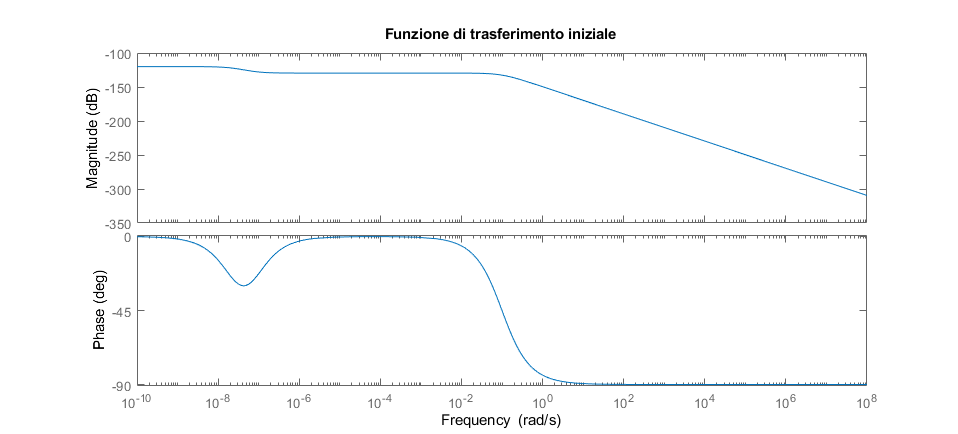
\includegraphics[width=1\textwidth]{fig1.png}
\caption{\label{fig:bode}Diagramma di Bode di $G(jw)$}
\end{figure}

\section{Il regolatore}
La funzione di trasferimento in anello aperto è definita come:
\[ L(s) = R(s) \cdot G(s)  \]
verrà ricavata tramite il calcolo di $R(s)$, composto dal regolatore statico $R_s(s)$ e dal regolatore dinamico $R_d(s)$, il regolatore richiesto deve rispettare i vincoli imposti ed essere fisicamente realizzabile.
\subsection{Regolatore Statico}

Dato che $\ G(s)$ non ha un polo nell'origine, per rispettare l'errore a regime nullo (1), è necessario inserirne uno. Considerando il guadagno del regolatore statico come  $ \mu_s =\num{e9}$ dB, otteniamo:

\[ R_s = \frac{\mu_s}{s}  \]


La funzione di trasferimento in serie con il regolatore statico risulta:
\[ G_e(s) = R_s(s) \cdot G(s) \]

\begin{figure}[!h]
\centering
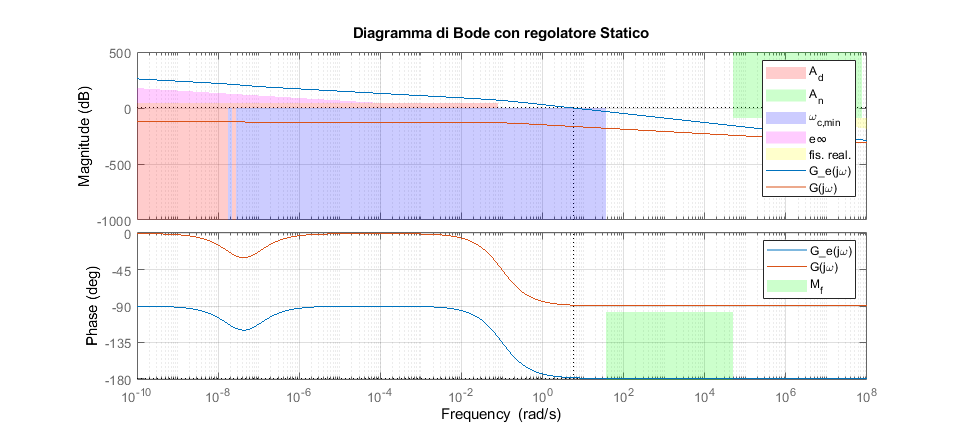
\includegraphics[width=1\textwidth]{fig2.png}
\caption{\label{fig:orbit}Diagramma di Bode di $G_e(jw)$ con vincoli}
\end{figure}

Si nota come non vengano rispettati i vincoli sui tempi di assestamento e sul margine di fase, che verranno fatte rispettare attraverso il regolatore dinamico.


\subsection{Regolatore Dinamico}
 La parte dinamica del regolatore deve rispettare determinate specifiche: il margine di fase $ Mf \geq 40\degree $ (2) per garantire un certo livello di robustezza del sistema regolato. 
La sovraelongazione percentuale massima che il sistema può accettare è $ S \leq 1\% $ (3). Il tempo di assestamento all' $ \epsilon\% $ deve essere inferiore a $ T_a,e=0,15s $ fissato (4).\\\\ Il disturbo sull'uscita $ d(t)$ con una banda limitata nel range di pulsazioni $[0.08]$, deve
essere abbattutto di almeno 45 dB (5).
Il rumore di misura $ n(t)$ con una banda limitata nel range di pulsazioni $[5\cdot10^4, 7.5\cdot10^7]$, deve
essere abbattutto di almeno 85 dB (6).

scriviscrivi
scriviscrivi
scrivi
scrivi

\section{Test del sistema di controllo sul modello lineare}


\end{document}